\chapter{Funciones de variable compleja}

En este capítulo se introducen nuevos conceptos como la holomorfía, aplicaciones conformes y más.

\section{Derivabilidad}

La definición de derivabilidad en $\C$ es practicamente indistinguible a la de $\R$.

\begin{definition}
    Sea $f : D \subseteq \C \to \C$ con $D$ abierto. Decimos que $f$ es \emph{derivable} en $z_0$ si existe
    \begin{equation*}
        f'(z_0) = \lim_{z \to z_0} \frac{f(z) - f(z_0)}{z - z_0}.
    \end{equation*}
\end{definition}

En general, vamos a identificar a $f: D \subseteq \C \to \C$ con la función $g: D' \subseteq \R^2 \to \R^2$ dada por
\begin{equation*}
    g(x, y) = (u(x, y), v(x, y)) = (\Re(f(x + iy)), \Im(f(x + iy))).
\end{equation*}
Sin embargo, usaremos de forma intercambiable ambas funciones, dado que gran parte de los conceptos son aplicables a las dos.

Tal como en $\R^2$ vale el álgebra de límites.

\begin{proposition}
    Sean $f: D \subseteq \C \to \C$ y $g: E \subseteq \C \to \C$ derivables (y que cumplan todas las hipótesis necesarias). Entonces,
    \begin{enumerate}
        \item $(f + g)' = f' + g'$.
        \item $(f \cdot g)' = f' \cdot g + f \cdot g'$.
    \end{enumerate}
\end{proposition}

Muchas veces vamos a querer escribir la derivabilidad de $f$ en $z_0$ de la siguiente manera equivalente: existe $L \in \C$ tal que para todo $\epsilon > 0$, existe $\delta > 0$ que cumple que 
\begin{equation*}
    \text{si } |z - z_0| < \delta, \text{ entonces } |f(z) - f(z_0) - L(z - z_0)| < |z - z_0| \epsilon.
\end{equation*}

A continuación probamos las condiciones de Cauchy--Riemann, que son extremadamente útiles para probar la derivabilidad de una función compleja.

\begin{proposition}[condiciones de Cauchy--Riemann]
    Sea $f : D \subseteq \C \to \C$ con $D$ abierto. Entonces, $f$ es derivable en $z_0 = x_0 + i y_0$ si y sólo si $u$ y $v$ son diferenciables en $(x_0, y_0)$ y
    \begin{equation*}
        \begin{cases}
            u_x (x_0, y_0) = v_y(x_0, y_0) \\
            u_y (x_0, y_0) = -v_x(x_0, y_0).
        \end{cases}
    \end{equation*}
\end{proposition}

\begin{proof}
    La demostración no es tan complicada, pero sí es bastante larga. Por lo tanto, no la incluyo acá. 
\end{proof}


\section{Holomorfía}

Definamos qué es una función holomorfa.

\begin{definition}
    Sea $f : D \subseteq \C \to \C$ con $D$ abierto. Decimos que $f$ es \emph{holomorfa} en $z_0$ si es derivable en algún entorno de $z_0$. Más en general, $f$ es holomorfa si es holomorfa en todo punto de su dominio.
\end{definition}

Llamamos \textit{dominio} a un conjunto a un conjunto abierto y conexo. Esto no se debe confundir con el dominio de una función, aunque usualmente terminan siendo lo mismo.

\begin{proposition}
    Sea $f : D \subseteq \C \to \C$ holomorfa, con $D$ dominio. Si $u(x, y)$ es constante, entonces $f$ es constante.
\end{proposition}

\begin{proof}
    Dado que $f$ es holomorfa, entonces se cumplen las condiciones de Cauchy--Riemann. Entonces,
    \begin{equation*}
        \begin{cases}
            0 = u_x (x_0, y_0) = v_y(x_0, y_0) \\
            0 = u_y (x_0, y_0) = -v_x(x_0, y_0).
        \end{cases}
    \end{equation*}
    Integrando las derivadas parciales, obtenemos que $u$ y $v$ son constantes y, por lo tanto, $f$ es constante.
\end{proof}

Otra propiedad útil.

\begin{proposition}
    Sea $f : D \subseteq \C \to \C$ holomorfa, con $D$ dominio. 
    Si $|f|$ es constante, entonces $f$ también lo es.
\end{proposition}

\begin{proof}
    Supongamos $|f(z)| = c$ para algún $c \geq 0$.  
    Si $c = 0$, entonces $f = 0$, que es constante.  

    Supongamos $c > 0$. Escribimos $f = u + iv$. La condición $|f|^2 = u^2+v^2 = c^2$ implica
    \begin{equation*}
        u u_x + v v_x = 0
        \quad\text{y}\quad
        u u_y + v v_y = 0.
    \end{equation*}
    Como $f$ es holomorfa, $u$ y $v$ satisfacen las ecuaciones de Cauchy–Riemann:
    \begin{equation*}
        u_x = v_y \quad\text{y}\quad u_y = -v_x.
    \end{equation*}
    Reemplazando, obtenemos
    \begin{equation*}
        u u_x + v v_x = u v_y - v u_y = 0,
    \end{equation*}
    \begin{equation*}
        u u_y + v v_y = -u v_x + v u_x = 0.
    \end{equation*}
    Es decir,
    \begin{equation*}
        \begin{cases}
            u v_y - v u_y = 0, \\
            -u v_x + v u_x = 0.
        \end{cases}
    \end{equation*}
    Esto significa que el determinante
    \begin{equation*}
        \begin{vmatrix}
            u & v \\
            u_x & v_x
        \end{vmatrix}
        = 0,
        \quad\text{y}\quad
        \begin{vmatrix}
            u & v \\
            u_y & v_y
        \end{vmatrix}
        = 0.
    \end{equation*}
    Como $u$ y $v$ no son ambas nulas, se deduce que $u_x=v_x=u_y=v_y=0$. sPor lo tanto $u,v$ son constantes, y en consecuencia $f$ es constante.
\end{proof}


\section{Funciones armónicas}

Más adelante veremos que una función sea holomorfa es condición suficiente para que sea infinitamente derivable. Por lo que, de ahora en adelatne, supondremos que las funciones $u: D \subseteq \R^2 \to \R$ y $v: D \subseteq \R^2 \to \R$ son infinitamente diferenciables.

\begin{definition}
    Sea $u: D \subseteq \R^2 \to \R$. Decimos que $u$ es \emph{armónica} si su laplaciano es nulo. Es decir,
    \begin{equation*}
        \Delta u = u_{xx} + u_{yy} = 0.
    \end{equation*}
\end{definition}

Consideremos ahora $f: D \subseteq \R^2 \to \R^2$ tal que $f(x, y) = u(x, y)+ i v(x, y)$. Nos interesa ver si $f$ es holomorfa.

\begin{definition}
    Sean $u, v: D \subseteq \R^2 \to \R$. Decimos que $v$ es una \emph{armónica conjugada} de $u$ si la función $f(x, y) = u(x, y) + i v(x, y)$ es holomorfa en todo su dominio.
\end{definition}

Probemos que siempre existe para dominios simplemente conexos y que es (casi) única.

\begin{proposition}
    Sea $u: D \subseteq \R^2 \to \R$ armónica, con $D$ simplemente conexo. Existe una armónica conjugada $v: D \subseteq \R^2 \to \R$ y está determinada de manera única salvo por una constante aditiva.
\end{proposition}

\begin{proof}
    Notemos primerarmente que la condición de Cauchy--Riemann es equivalente a pedir que 
    \begin{equation*}
        \nabla v = (-u_y, u_x).
    \end{equation*}
    Por lo tanto, basta con encontrar una función $v$ que cumpla. 

    Dado que nuestro dominio es simplemente conexo, el campo vectorial $(-u_y, u_x)$ es el gradiente de una función $v$ si y sólo si el rotor del campo es nulo. Entonces,
    \begin{equation*}
        \nabla \times (-u_y, u_x) = u_{xx} - (-u_{yy}) = u_{xx} + u_{yy} = 0,
    \end{equation*}
    dado que $u$ es armónica.
\end{proof}

\begin{proposition}
    Sea $f: D \subseteq \C \to \C$ holomorfa con $D$ dominio. Si $\Im f$ está contenida en una recta, entonces $f$ es constante.
\end{proposition}

\begin{proof}
    Sea $f(x, y) = u(x, y) + i v(x, y)$ tal que cumple las hipótesis e $\Im f$ está contenida en una recta. Entonces, existen $a, b, c \in \R$, donde $a$ y $b$ no son ambos nulos, tales que todo $(x, y) \in \R^2$ cumple
    \begin{equation*}
        a u(x, y) + b u(x, y) = c.
    \end{equation*}

    Tomamos derivadas parciales respecto a $x$ e $y$:
    \begin{equation*}
        \begin{cases}
            a u_x(x, y) + bv_x(x, y) = 0 \\
            a u_y(x, y) + bv_y(x, y) = 0. \\
        \end{cases}
    \end{equation*}
    Como $f$ es holomorfa, aplicamos Cauchy--Riemann, entonces
    \begin{equation*}
        \begin{cases}
            a u_x(x, y) + bv_x(x, y) = 0 \\
            -a v_x(x, y) + bu_x(x, y) = 0. \\
        \end{cases}
    \end{equation*}
    Finalmente, escribimos al sistema en forma matricial:
    \begin{equation*}
        \begin{pmatrix}
            a & b \\
            b & -a 
        \end{pmatrix}
        \begin{pmatrix}
            u_x \\
            v_x
        \end{pmatrix}
        =
        \begin{pmatrix}
            0 \\
            0
        \end{pmatrix}.
    \end{equation*}
    El determinante de la matriz es $-a^2 - b^2 \neq 0$. Por ende, $u_x = v_x = 0$ y, por Cauchy--Riemann, $u_y = v_y = 0$.
\end{proof}


\section{Transformaciones conformes}

Las \textit{transformaciones conformes} en esencia son funciones que preservan ángulos. Veamos qué quiere decir esto.

\begin{definition}
    Decimos que $f: D \subseteq \R^2 \to \R^2$ es una \emph{transformación conforme} si dado un par de curvas $\gamma, \sigma : [a, b] \to R^2$ que intersecan en $z_0$ con un ángulo $\alpha$, la imagen por $f$ preserva el mismo ángulo.
\end{definition}

Para entender un poco mejor, veamos un ejemplo gráfico:

\begin{figure}[H]
\centering
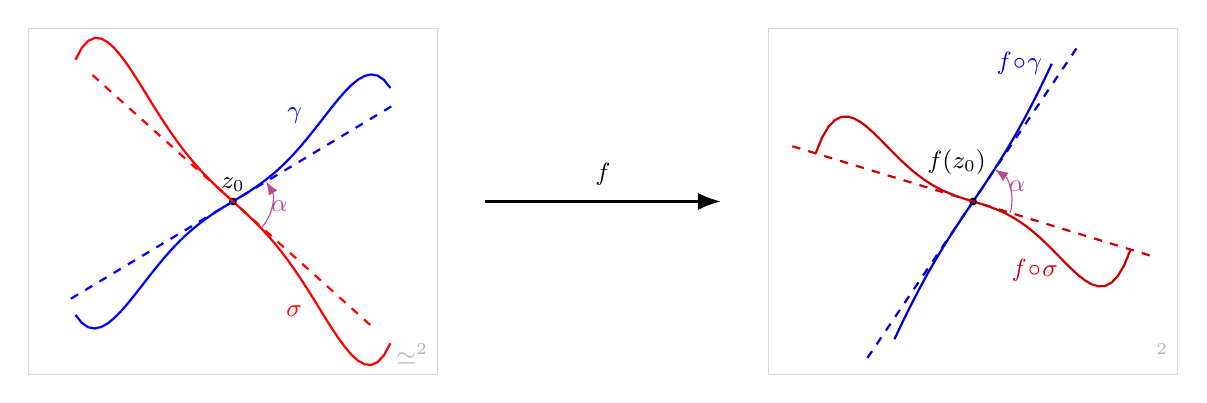
\begin{tikzpicture}[
    scale=1.0,
    >=Latex,
    every node/.style={font=\small},
]
\usetikzlibrary{arrows.meta,angles,quotes}

% ====== Parámetros ======
\pgfmathsetmacro{\mone}{0.6}    % pendiente de gamma en z0
\pgfmathsetmacro{\mtwo}{-0.9}   % pendiente de sigma en z0
\pgfmathsetmacro{\cA}{0.35}     % curvatura cúbica gamma
\pgfmathsetmacro{\cB}{0.40}     % curvatura cúbica sigma
\pgfmathsetmacro{\dA}{-0.08}    % curvatura quíntica gamma
\pgfmathsetmacro{\dB}{0.10}     % curvatura quíntica sigma

% Rotación local (diferencial de f)
\pgfmathsetmacro{\phi}{25}      

% Ángulos
\pgfmathsetmacro{\thone}{atan(\mone)}
\pgfmathsetmacro{\thtwo}{atan(\mtwo)}
\pgfmathsetmacro{\thonep}{\thone + \phi}
\pgfmathsetmacro{\thtwop}{\thtwo + \phi}

% Pendientes rotadas
\pgfmathsetmacro{\monep}{tan(\thonep)}
\pgfmathsetmacro{\mtwop}{tan(\thtwop)}
\pgfmathsetmacro{\cAp}{0.35}
\pgfmathsetmacro{\cBp}{0.40}
\pgfmathsetmacro{\dAp}{-0.08}
\pgfmathsetmacro{\dBp}{0.10}

% Largo tangentes
\pgfmathsetmacro{\L}{2.4}

% ====== Panel izquierdo ======
\begin{scope}[shift={(-4.7,0)}]
  \draw[gray!30] (-2.6,-2.2) rectangle (2.6,2.2);
  \node[anchor=south east,gray!60] at (2.6,-2.2) {$\C \simeq \R^2$};

  \coordinate (Z0) at (0,0);

  % Curva gamma con x^3 y x^5
  \draw[thick,blue,domain=-2:2,samples=50]
    plot (\x, {\mone*\x + \cA*\x^3 + \dA*\x^5});
  \node[blue,above left] at (1,{\mone*1 + \cA*1 + \dA*1}) {$\gamma$};

  % Curva sigma con x^3 y x^5
  \draw[thick,red,domain=-2:2,samples=50]
    plot (\x, {\mtwo*\x - \cB*\x^3 + \dB*\x^5});
  \node[red,below left] at (1,{\mtwo*1 - \cB*1 + \dB*1}) {$\sigma$};

  % Punto z0
  \fill (Z0) circle (1.4pt) node[above] {$z_0$};

  % Tangentes verdaderas
  \draw[dashed,blue,thick]
    ({-\L*cos(\thone)},{-\L*sin(\thone)}) -- ({\L*cos(\thone)},{\L*sin(\thone)});
  \draw[dashed,red,thick]
    ({-\L*cos(\thtwo)},{-\L*sin(\thtwo)}) -- ({\L*cos(\thtwo)},{\L*sin(\thtwo)});

  % Ángulo alpha
  \coordinate (Tg) at ({cos(\thone)},{sin(\thone)});
  \coordinate (Ts) at ({cos(\thtwo)},{sin(\thtwo)});
  \pic[draw,->,blue!40!red!70,angle radius=14pt,"$\alpha$",angle eccentricity=1.2]
      {angle = Ts--Z0--Tg};
\end{scope}

% Flecha
\draw[very thick,->] (-1.5,0) -- (1.5,0) node[midway,above=2pt] {$f$};

% ====== Panel derecho ======
\begin{scope}[shift={(4.7,0)}]
  \draw[gray!30] (-2.6,-2.2) rectangle (2.6,2.2);
  \node[anchor=south east,gray!60] at (2.6,-2.2) {$\R^2$};

  \coordinate (W0) at (0,0);

  % Imagen gamma con curvatura
  \draw[thick,blue!80!black,domain=-1:1,samples=50]
    plot (\x, {\monep*\x + \cAp*\x^3 + \dAp*\x^5});
  \node[blue!80!black,left] at (1,{\monep*1 + \cAp*1 + \dAp*1}) {$f\!\circ\!\gamma$};

  % Imagen sigma con curvatura
  \draw[thick,red!80!black,domain=-2:2,samples=50]
    plot (\x, {\mtwop*\x - \cBp*\x^3 + \dBp*\x^5});
  \node[red!80!black,below left] at (1.2,{\mtwop*1 - \cBp*1 + \dBp*1}) {$f\!\circ\!\sigma$};

  % Punto f(z0)
  \fill (W0) circle (1.4pt) node[above, yshift=6pt, xshift=-6pt] {$f(z_0)$};

  % Tangentes
  \draw[dashed,blue!80!black,thick]
    ({-\L*cos(\thonep)},{-\L*sin(\thonep)}) -- ({\L*cos(\thonep)},{\L*sin(\thonep)});
  \draw[dashed,red!80!black,thick]
    ({-\L*cos(\thtwop)},{-\L*sin(\thtwop)}) -- ({\L*cos(\thtwop)},{\L*sin(\thtwop)});

  % Ángulo alpha
  \coordinate (Tgp) at ({cos(\thonep)},{sin(\thonep)});
  \coordinate (Tsp) at ({cos(\thtwop)},{sin(\thtwop)});
  \pic[draw,->,blue!40!red!70,angle radius=14pt,"$\alpha$",angle eccentricity=1.2]
      {angle = Tsp--W0--Tgp};
\end{scope}
\end{tikzpicture}
\end{figure}


Decimos que, en particular, esta transformación es conforme en $z_0$. Notemos que las tangentes a las curvas $\gamma$ y $\sigma$ forman un ángulo $\alpha$ y, luego de aplicar $f$, aún se preserva el ángulo.

Las transformaciones conformes elementales en $\R^n$ son:
\begin{enumerate}
    \item \textbf{Homotecias:} $f(x) = \lambda x$, con $\lambda \in \R_{>0}$.
    \item \textbf{Traslaciones:} $f(x) = x + a$, con $a \in \R^n$.
    \item \textbf{Ortogonales:} $f(x) = A x$, donde $A \in O(n)$.
    \item \textbf{Inversiones:} $f(x) = \dfrac{x}{\|x\|^2}$.
\end{enumerate}


Toda transformación conforme en $\R^n$ ($n \geq 3$) se obtiene como composición de estas transformaciones ---esto es el teorema de Liouville, pero por ahora no lo demostramos---.

\bigskip

Consideremos las trasformaciones $T: \R^2 \to \R^2$ lineales conformes. Es decir, las que cumplen
\begin{equation*}
    \frac{Tv \cdot Tw}{\Vert Tv \Vert \, \Vert Tw \Vert} = \frac{v \cdot w}{\Vert v \Vert \, \Vert w \Vert}.
\end{equation*}
En particular, las transformaciones ortogonales preservan el producto interno y, por lo tanto, los ángulos.

\begin{proposition}
    Sea $T: \R^2 \to \R^2$ una transformación. Entonces, $T$ es conforme si y sólo si $T = \lambda U$ con $U$ ortogonal.
\end{proposition}

\begin{proof}
    ($\Rightarrow$) Sea $T$ conforme y sea $\{v, w\}$ una base ortonormal de $\R^2$. Por conformidad de $T$, $\{Tv, Tw\}$ es ortogonal. Calculamos
    \begin{align*}
        (v + w) \cdot (v - w) &= \Vert v \Vert^2 - \Vert w \Vert^2 \\
        &= 1 - 1 \\
        &= 0.
    \end{align*}
    Recordemos que el producto interno entre dos vectores es el producto entre las normas y coseno del ángulo; por lo tanto, por conformidad, 
    \begin{align*}
        0 = T(v + w) \cdot T(v - w) &= (Tv + Tw) \cdot (Tv - Tw) \\
        &= \Vert Tv \Vert^2 - \Vert Tw \Vert^2.
    \end{align*}
    Entonces, $\Vert Tv \Vert = \Vert Tw \Vert$. Con definir $U = \Vert Tv \Vert^{-1} T$ obtenemos una transformación ortonormal.

    Como $T = \lambda U$ con $\lambda = \Vert Tv \Vert$ y $U$ ortogonal, queda probada la implicación.

    ($\Leftarrow$) Es inmediato.
\end{proof}

Una función $f: \R^2 \to \R^2$ es un \emph{difeomorfismo} si es diferenciable, biyectiva y su inversa es diferenciable.

\begin{proposition}
    Sea $f: D \subseteq \R^2 \to \R^2$ un difeomorfismo con $D$ dominio. Entonces, $f$ es conforme si y sólo si $f$ es holomorfa o $\overline{f}$ es holomorfa.
\end{proposition}

\begin{proof}
    No lo probamos.
\end{proof}

\begin{theorem}
    Sea $f: D \subseteq \R^2 \to \R^2$ conforme. Entonces, $f$ puede escribirse como composición de a lo sumo una traslación, una homotecia, una transformación ortogonal
    y una inversión.
\end{theorem}

\begin{proof}
    Ídem.
\end{proof}

\begin{proposition}
    Sea $D \subseteq \C$, $f : D \to \C$ y $z_0 \in D^\circ$. 
    Si $f$ es holomorfa en $z_0$ y $f'(z_0) \neq 0$, entonces $f$ es conforme en $z_0$.
\end{proposition}

\begin{proof}
    Escribimos $f=u+iv$ con $u,v:D\to\R$ de clase $C^1$ cerca de $z_0$. 
    Como $f$ es holomorfa en $z_0$, satisface las ecuaciones de Cauchy--Riemann en $z_0$:
    \begin{equation*}
        u_x(z_0)=v_y(z_0), \qquad u_y(z_0)=-\,v_x(z_0).
    \end{equation*}
    El jacobiano en $z_0$ es
    \begin{equation*}
        Df(z_0)=\begin{pmatrix} u_x & u_y \\ v_x & v_y \end{pmatrix}_{z_0}
                =\begin{pmatrix} u_x & -v_x \\ v_x & u_x \end{pmatrix}_{z_0}.
    \end{equation*}
    Sea $f'(z_0)=a+ib$ (con $a=u_x(z_0)$ y $b=v_x(z_0)$). Entonces
    \begin{equation*}
        Df(z_0)=\begin{pmatrix} a & -b \\ b & a \end{pmatrix}.
    \end{equation*}
    Esta matriz es, en notación real, la multiplicación compleja por $a+ib$. Descompone como
    \begin{equation*}
        \begin{pmatrix} a & -b \\ b & a \end{pmatrix}
        = \sqrt{a^2+b^2}\;
        \begin{pmatrix} \cos\theta & -\sin\theta \\ \sin\theta & \cos\theta \end{pmatrix},
        \qquad \theta=\arg(a+ib).
    \end{equation*}
    Es decir, $Df(z_0)$ es una homotecia de razón $\lambda=\lvert f'(z_0)\rvert>0$ seguida de una rotación. 
    Por lo tanto, $Df(z_0)$ preserva ángulos y orientaciones. En consecuencia, $f$ es conforme en $z_0$.
\end{proof}



\section{Funciones elementales}

Nos hacemos la siguiente pregunta: dada una función en los reales, ¿existe una función compleja tal que la extiende?

\begin{definition}
    Sea $f : A \subseteq \R \to \R$. Decimos que $g: D \subseteq \C \to \C$ es una \emph{extensión al plano complejo} de $f$ si $g|_A = f$.
\end{definition}

Las extensiones de algunas funciones típicas a $\C$ son:
\begin{enumerate}
    \item Exponencial:
    \begin{equation*}
        e^z = e^x(\cos y + i \sin y), \quad z = x + i y.
    \end{equation*}
    \item Seno:
    \begin{equation*}
        \sin z = \frac{e^{iz} - e^{-iz}}{2i}.
    \end{equation*}
    \item Coseno:
    \begin{equation*}
        \cos z = \frac{e^{iz} + e^{-iz}}{2}.
    \end{equation*}
    \item Tangente:
    \begin{equation*}
        \tan z = \frac{\sin z}{\cos z}.
    \end{equation*}
\end{enumerate}

Si intentamos extender $\log$ nos vamos a encontrar con un problema. Sea $w \in \C$. Buscamos $z \in \C$ tal que 
\begin{equation}
    \label{eq:expo-inv}
    e^z = w.
\end{equation}
Primero, aplicamos módulo a la ecuación \ref{eq:expo-inv} y obtenemos
\begin{equation*}
    |w| = |e^z| = e^x.
\end{equation*}
Además, tomando argumento obtenemos
\begin{equation*}
    \arg w = \arg(e^z) = y + 2 \pi k, \quad k \in \Z.
\end{equation*}
Acá nos encontramos con el primer problema: hay múltiples elecciones para el arguento. Para resolver esto, se restringe el el argumento a $( -\pi, \pi]$. A la función
\begin{equation*}
    \Arg(z) = \begin{cases}
        \arccos \left(\frac{x}{\sqrt{x^2 + y^2}}\right) & \text{si } y \geq 0, \\
        -\arccos \left(\frac{x}{\sqrt{x^2 + y^2}}\right) & \text{si } y < 0,
    \end{cases}
\end{equation*}
se le llama el \textit{argumento principal}. 

De vuelta, nos encontramos con otro problema: el argumento principal no es continua en la semirrecta real negativa. Más adelante podemos probar que, no importa como definamos la extensión, es imposible extender de forma continua el logaritmo a todo $\C \setminus \{0\}$. No obstante, si consideramos el dominio $\C \setminus \{ x + 0 \cdot i  \mid x < 0\}$, la extensión es continua.

\begin{definition}
    Definimos el \emph{logaritmo principal} como
    \begin{equation*}
        \Log(z) = \ln|z| + i \Arg(z), \qquad z \in \C \setminus \{x \leq 0\}.
    \end{equation*}
\end{definition}